% Roll no 33, Haseeb Rahman
\textbf{\textcolor{LightMagenta}{ Why does a single perceptron cannot simulate simple XOR function? Explain how this limitation is overcome? (Dec 2019) \hfill 4 marks}} \\[5pt]

\textcolor{purple}{\underline{Perceptron}} \\
The perceptron can be represented by the schematic shown in the figure below.
\begin{center}
    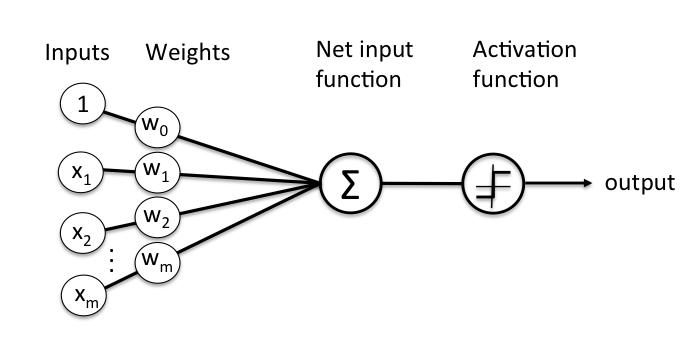
\includegraphics[width=.8\textwidth]{Images/A22_img1.png}
\end{center}
\\
As we can see, it calculates a weighted sum of its inputs and thresholds it with a step function. Geometrically, this means the perceptron can separate its input space with a hyperplane. That’s where the notion that a perceptron can only separate linearly separable problems came from. Since the XOR function is not linearly separable, it really is impossible for a single hyperplane to separate it.
\\
\begin{center}
    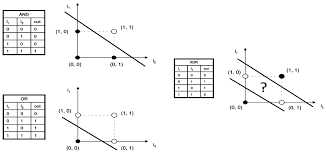
\includegraphics{Images/A22_img2.png}
\end{center}
\\
So, a single perceptron cannot simulate simple XOR function.
\\
The delta rule is used when the training
data set is not linearly separable.
\\
\textcolor{purple}{\underline{Gradient Descent and Delta Rule}} \\
The technique used to determine how much a weight should be changed is known
as gradient descent method. At every stage of the computation, the error is a
function of the weights. If we plot the error against the weights, we get a higher
dimensional analog of something like a curve or surface. At any point on this surface,
the gradient suggests how steeply the error will be reduced or increased for a change
in the weight. The algorithm will attempt to change the weights that result in the
greatest reduction in error.
\\
A simplified model of the error surface showing the direction of gradient.
\begin{center}
    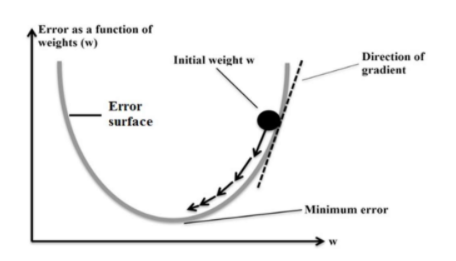
\includegraphics[width=.8\textwidth]{Images/A22_img3.png}
\end{center}

The method used to calculate the adjusted weights is known as the delta rule.
\\
The rule for computing the adjusted weights can be succinctly stated as follows. Let w be the weight and $w^+$ its adjusted weight. Let E be the total sum of squares of errors . Then $w^+$ is computed by 
\begin{center}
  \[ w^+ = w-\eta\frac{\partial E}{\partial w}
\]  
\end{center}
\\
Here $\frac{\partial E}{\partial w}$ is the gradient of E with respect to w; that is, the rate at which E is changing with respect to (The set of all such gradients specifies the direction in which E is decreasing the most rapidly, that is, the direction of quickest descent.)